\section{Kwadratury elementarne}
%%%%%%%%%%%%%%%%%%%%%%%%%
	\begin{frame}{Wzór prostokątów}
      	\begin{center}
      		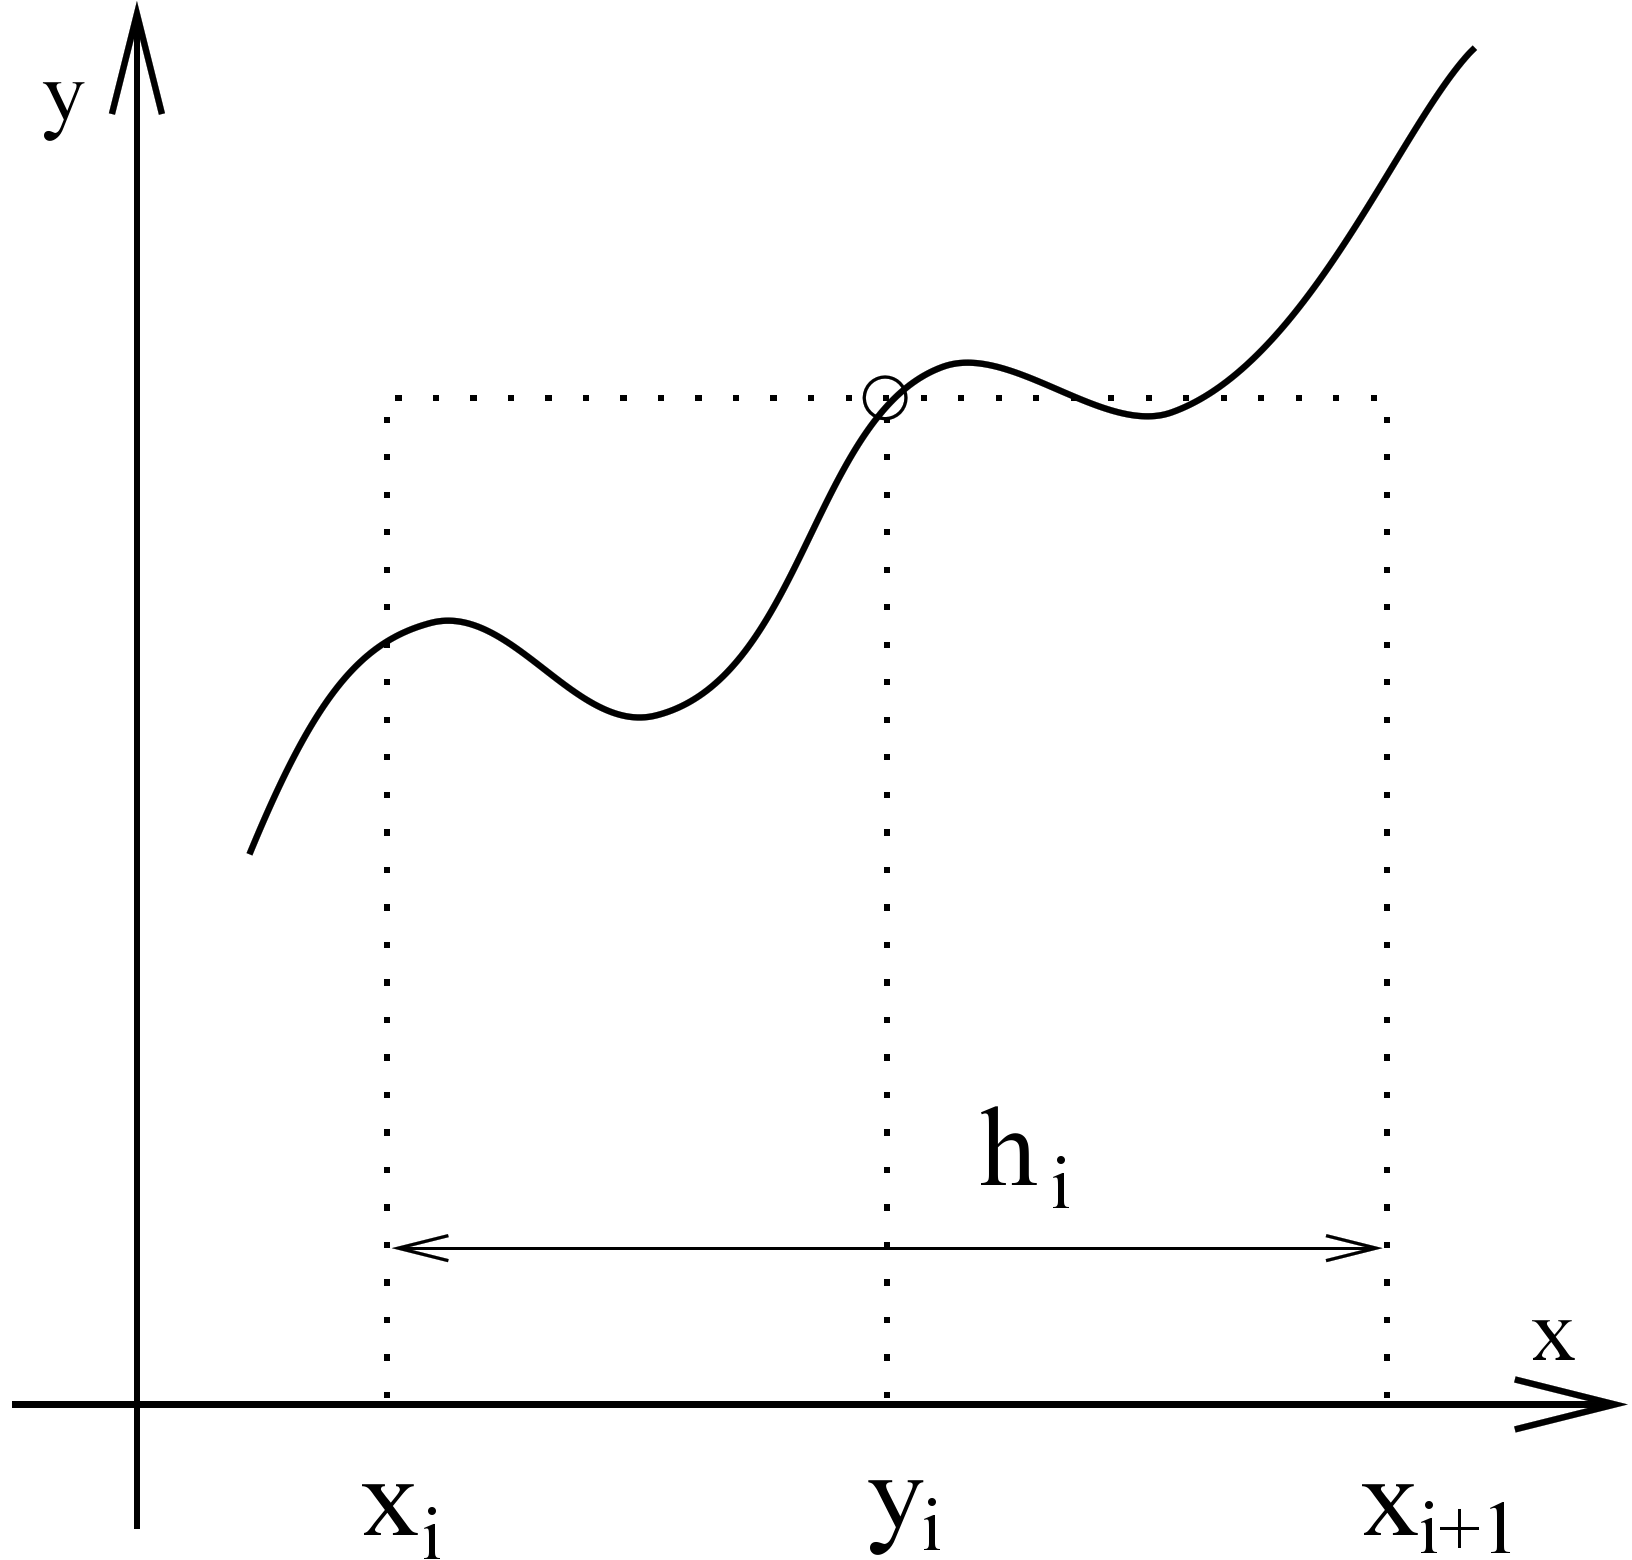
\includegraphics[width=0.4\linewidth]{img/6/image002.png}
      	\end{center}
        
		$$
y_{i}= \frac{1}{2}(x_{i}+x_{i+1}),\ \ \ f(x)=f(y_{i})+ \sum_{p=1}^{\infty}\frac{(x-y_{i})^{p}}{p!}f^{(p)}(y_{i})
		$$
        
		$$
\int_{xi}^{x_{i+1}}f(x)dx=\underbrace{(y_{i})h_{i}}_{R}+\frac{1}{24}h_{i}^{3}f''(y_{i})\tilde{R}+\frac{1}{1920}h_{i}^{5}f^{(4)}(y_{i})+\ldots
		$$
	\end{frame}
%%%%%%%%%%%%%%%%%%%%%%%%%
	\begin{frame}{Wzór trapezów}
    	$$
f(x_{i})=f(y_{i})- \frac{1}{2}h_{i}f'(y_{i})+\ldots,\ \ f(x_{i+1})=f(y_{i})+ \frac{1}{2}h_{i}f'(y_{i})+\ldots
        $$
        
		$$
\int_{a}^{b}f(x)dx=\underbrace{\frac{1}{2}[f(x_{i}) + f(x_{i+1})] \cdot h_{i}}_{T} - \frac{1}{12}h_{i}^{3} f''(y_{i})-\frac{1}{480}h_{i}^{5}f^{(4)}(y_{i})+\ldots
		$$ 
	\end{frame}
%%%%%%%%%%%%%%%%%%%%%%%%%
	\begin{frame}{Wzór Simpsona}
		$$
        \textnormal{sposób:} \left\{\begin{array}{l}
  			I = R + E + F \\
        	I = T - 2E - 4F
        \end{array}\right.
        $$
        
        $$
S = \frac{1}{6}h_{i}[f(x_{i})+4f(\frac{x_{i}+x_{i+1}}{2})+f(x_{i+1})];\ E=-\frac{1}{2880}h_{i}^{5}f^{(4)}(y_{i})
		$$
        oparta na interpolacji 2-go rzędu\newline ale dokładna dla funkcji sześciennych.
        
      	\begin{center}
      		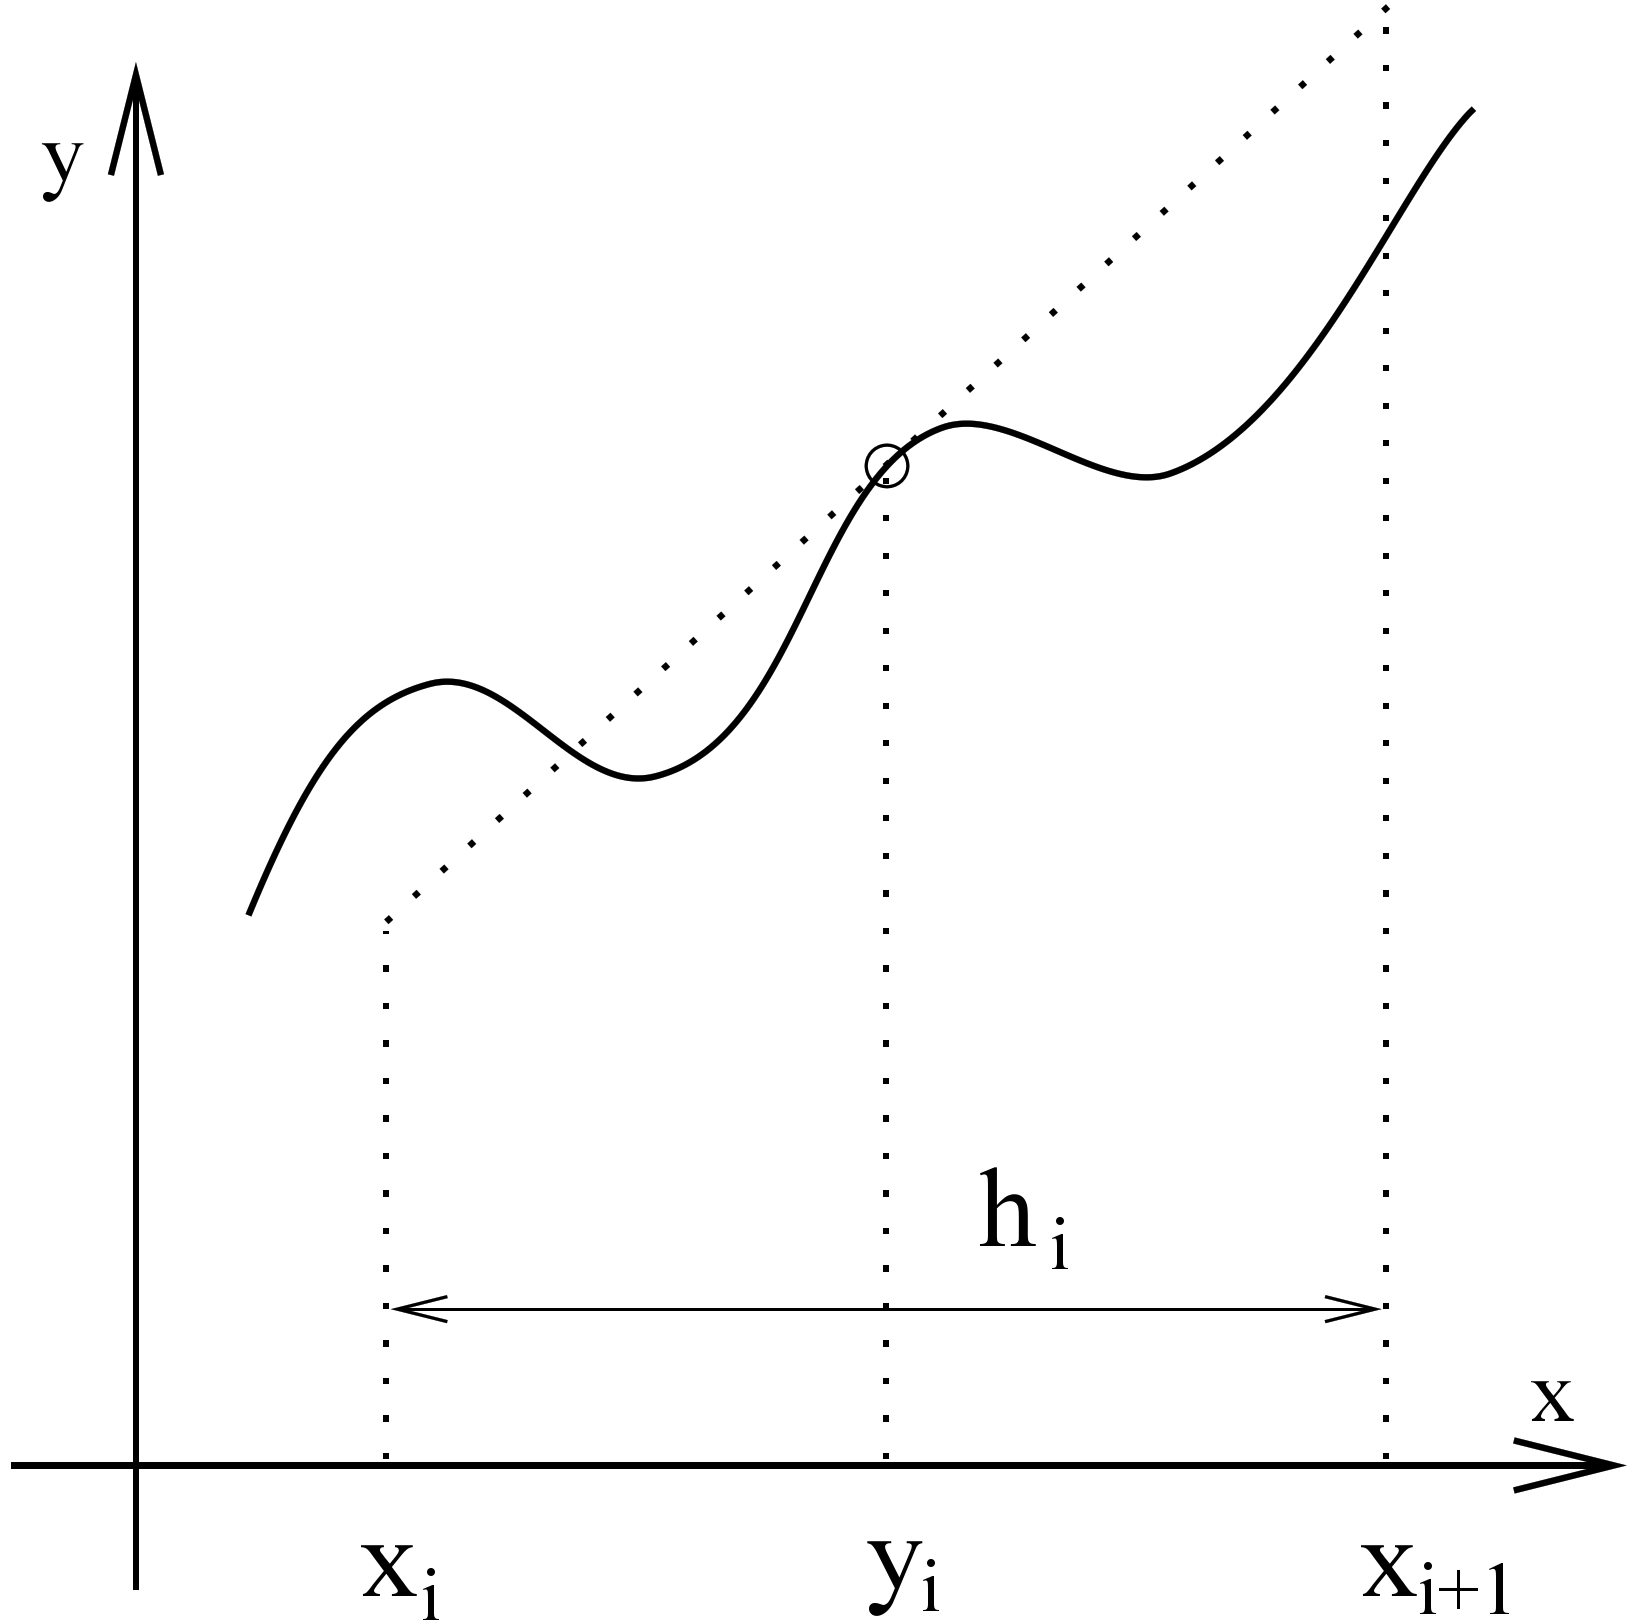
\includegraphics[width=0.35\linewidth]{img/6/image003.png}
      	\end{center}
	\end{frame}
%%%%%%%%%%%%%%%%%%%%%%%%%
